\section{Iconic semantics for modal verbs}

In this sketch I want to deal with certain modal verbs: that means those of cognition and perception like to think and see, and the sketch will taper out towards some modal auxiliaries like wanting. These kinds of verbs are roughly characterised as requiring copies of entities to be instantiated in worlds similar to but not exactly that of whatever base narrative reality is referred to in the discourse. For example, in \texttt{Alice sees Bob drink a beer, Bob drinks another after Alice leaves.}, there are two Bobs, because the one in Alice's mental-theatre drinks a single beer, and the one in the base reality of the narration drinks two. So there are two worlds $\mathfrak{W}$ here, one basic, and a $\mathfrak{W}_{\texttt{A}}$ for the world in Alice's perception. Things get intractably tricky fairly quickly with these modals: to do epistemic logic means to have nested indices of what Alice thinks Bob thinks Alice thinks, to gossip is to reason about he-said-she-said, to understand complex narratives is to reason about stories-told-within-stories, and counterfactuals are a whole thing too. So that is a fundamental mystery: all this seems fairly complicated to encode and reason about symbolically, but it is phenomenologically fairly easy for adults to do, so what gives? What sort of mathematical presentation of these modals would at least reflect this lightness and ease?

I think thought-bubbles that show up in comic books are a pretty good start. Their cloudlike shape is a visual convention indicating a separate mental world, and they are typically used to represent want when the contents are also iconic representations.

\begin{figure}[h!]
    \centering
    \begin{minipage}[b]{0.4\textwidth}
        \centering
        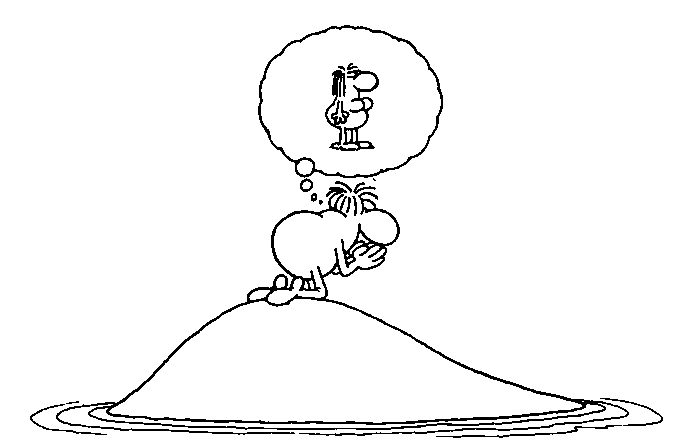
\includegraphics[height=4cm]{figures/bubbles/companion}
        \label{fig:companion}
    \end{minipage}
    \hfill
    \begin{minipage}[b]{0.4\textwidth}
        \centering
        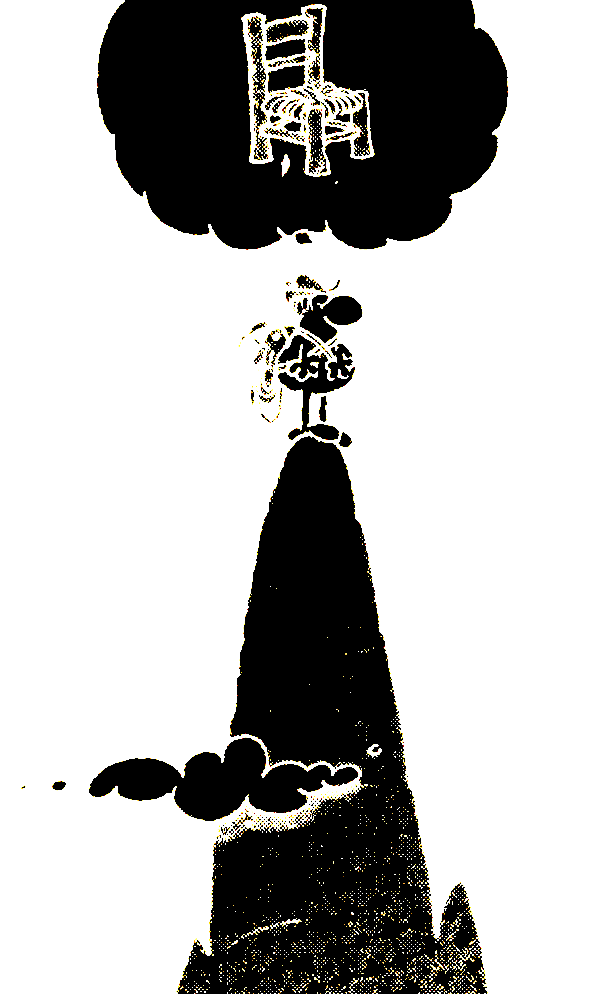
\includegraphics[height=4cm]{figures/bubbles/chair}
        \label{fig:chair}
    \end{minipage}
    \caption{Two examples by Mordillo, an artist I liked as a child: a thought bubble representing a woman, where the context of a stranded man implies a want for companionship, and a thought bubble representing a chair, where the context of a climber on a tall summit implies a want for rest.}
    \label{fig:mordillo}
\end{figure}

The visual convention for cognitive and perceptive-alethic verbs is, as far as I can tell, a kind of x-ray effect into the contents of a head, which employs the familiar container metaphor: the head is a container for thoughts.

\begin{figure}[h!]
    \centering
    \begin{minipage}[b]{0.4\textwidth}
        \centering
        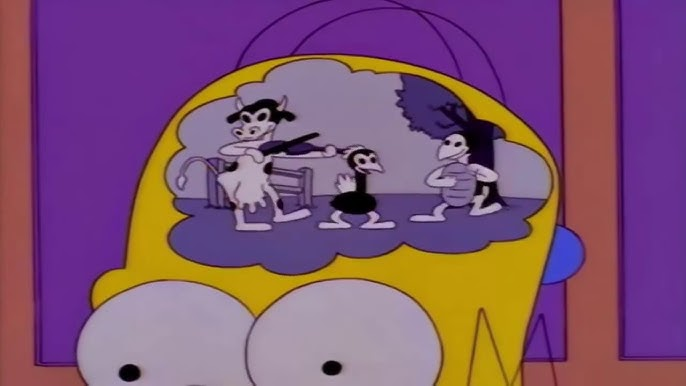
\includegraphics[height=4cm]{figures/bubbles/homer}
        \label{fig:homer}
    \end{minipage}
    \hfill
    \begin{minipage}[b]{0.4\textwidth}
        \centering
        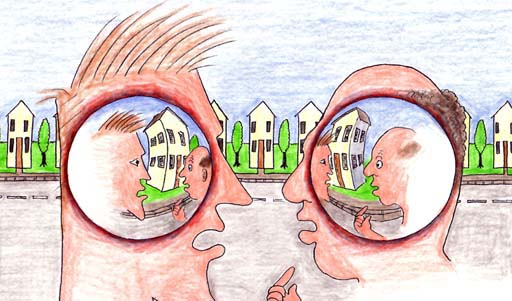
\includegraphics[height=4cm]{figures/bubbles/nestedminds}
        \label{fig:lehar}
    \end{minipage}
    \caption{On the left, a scene from the Simpsons showing the contents of Homer's mental-theatre. On the right, a depiction of two separate mental-theatres with a fisheye effect, taken from Steven Lahars "A Cartoon Epistemology" freely available online, which was also the initial inspiration for this sketch.}
    \label{fig:thinking}
\end{figure}

\begin{figure}[h!]
    \centering
    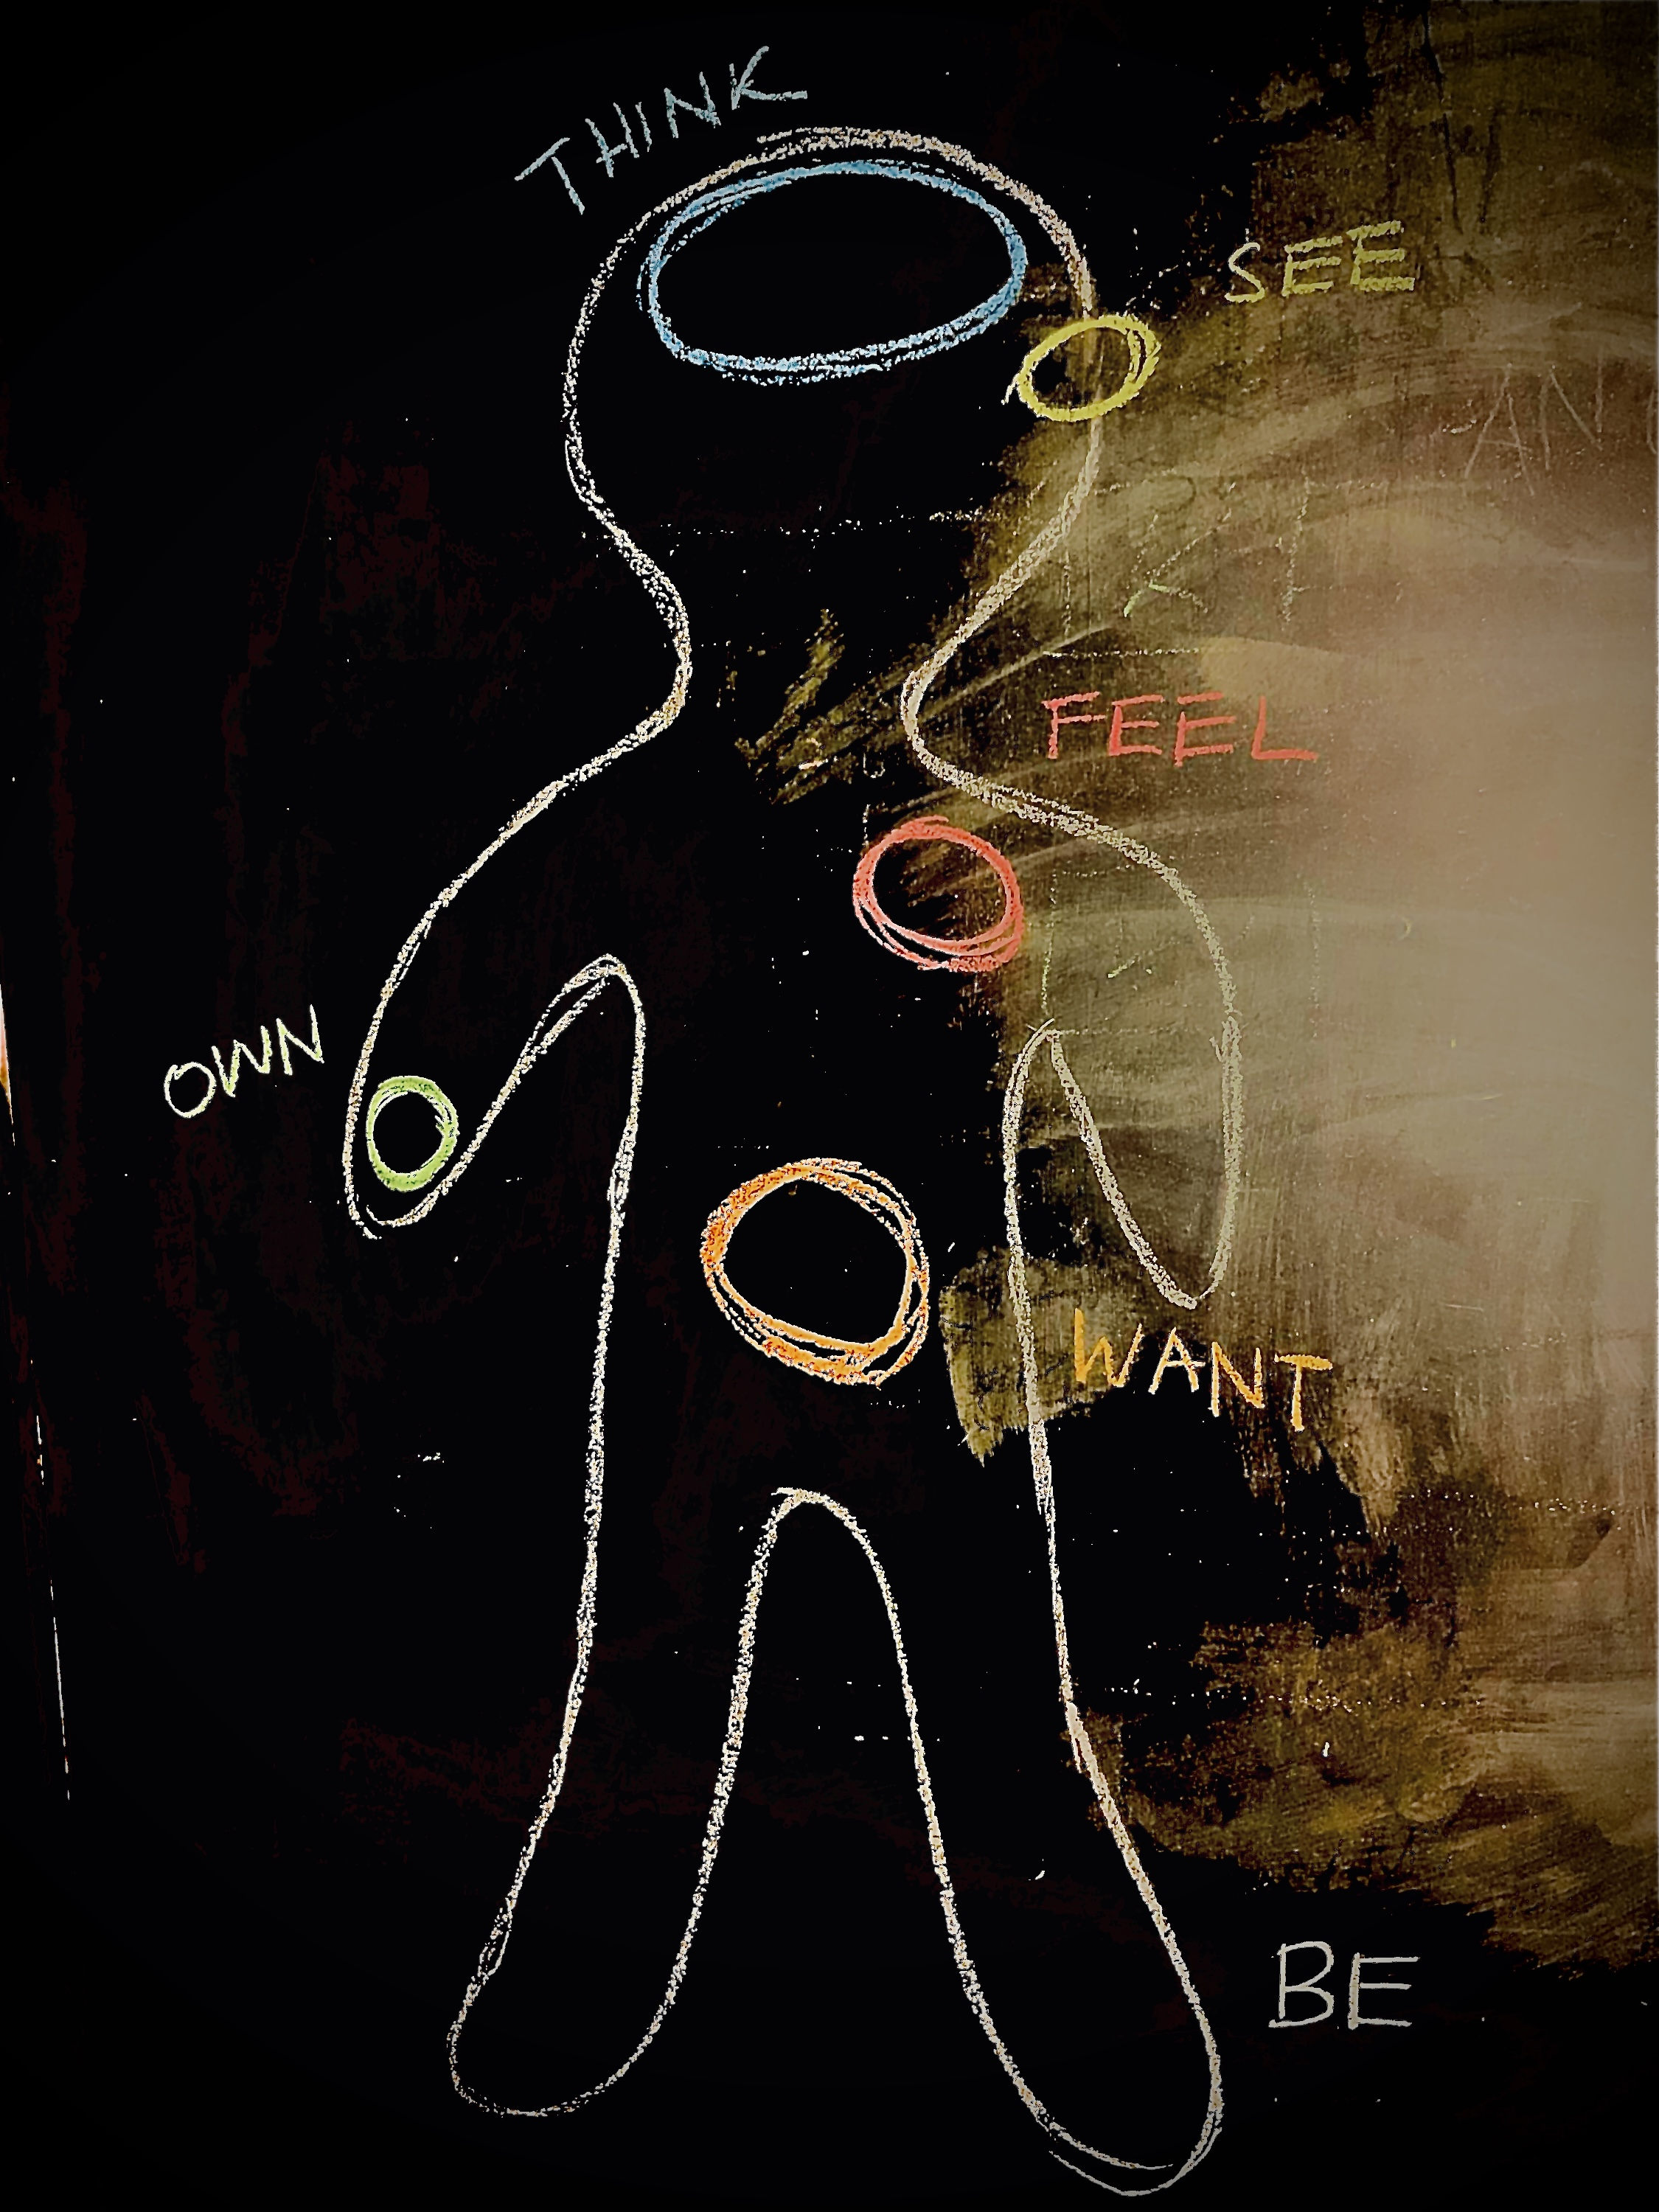
\includegraphics[height=9cm]{figures/bubbles/creepy}
    \caption{So the basic idea is to put representations of worlds inside bounded regions as containers, and in this way iconic semantics provides a univocal setting that displays all of the relevant worlds at once. We are free to pick visual conventions, as they are no more or less arbitrary than the assignment of indices and symbols such as $\mathfrak{W}_{\texttt{A}}$ to the contents of possible worlds. Here is a sketch convention for containers on an iconic representation of a person for different modal verbs: seeing, thinking, feeling, owning, and wanting. I sent this excitedly with little supporting context to Bob while I was writing my thesis. He was concerned. Then I got concerned. Childlike became creepy, and neither are good looks. I think I have supplied enough context to make this sensible, but there's no way I'm going to beat the crazy allegations.}
    \label{fig:creepy}
\end{figure}

For alethic verbs in particular (those modals that are truth-preserving, in that they "do not forget" the truth), there's a need for the contents of the container to be synchronised with the contents of the outside world. Here are some observations that enable this in \textbf{Contrel}. The basic enabling insight is that, in Euclidean spaces, if we have a hollow container with a solid blob inside, there's an approximately continuous bijection between the (open set) insides of the container and the outside world.

\clearpage

\begin{figure}[h!]
\centering
\[\scalebox{0.75}{\tikzfig{bubbles/container}}\]
\caption{The inside and the outside of a container with a solid blob inside are both homotopic to the space with a puncture. This is only approximately a continuous bijection because the unbounded outside space can only map to the open interior of the container. We can use such bijections as a bridge to establish connections between elements of different possible worlds.}
\label{fig:creepy}
\end{figure}

The second, and unfinished, idea is that if we have a handle on the individual components of sticky spiders, then we may use something like a very-well-behaved lens (hence its occurrence in the introduction) to ensure that the inside of the container is really behaving like a faithful storage medium for the goings-on outside. I think that's suggestive enough, and I'll deal with parthood in the next sketch. The last thing I want to deal with here is the problem of infinite regress for epistemic modals like knowing: if I know something, then I know I know it, and I know I know I know it, and so on. A na\"{i}ve solution is to just use an infinitely-nested series of containers.

\begin{figure}[h!]
\centering
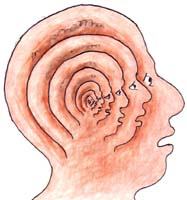
\includegraphics[height=5cm]{figures/bubbles/infinity}
\caption{Again from Cartoon Epistemology, on the unsatisfactory nature of infinitely-nested containers: \emph{But who is the viewer of this internal theatre of the mind? For whose benefit is this internal performance produced? Is it the little man at the center who sees this scene? But then how does HE see? Is there yet another smaller man inside that little man's head, and so on to an infinite regress of observers within observers?}}
\label{fig:infinity}
\end{figure}

\clearpage

So the problem here is how to encode this infinite regress with finite means in an iconic model. The usual monadic approach still runs into the problem that you have to map a potential nested-infinity of possible worlds onto some finite model if one cares about cognitive realism. In iconic semantics, we can modify the space itself; here I think Escher was onto something.

\begin{figure}[h!]
\centering
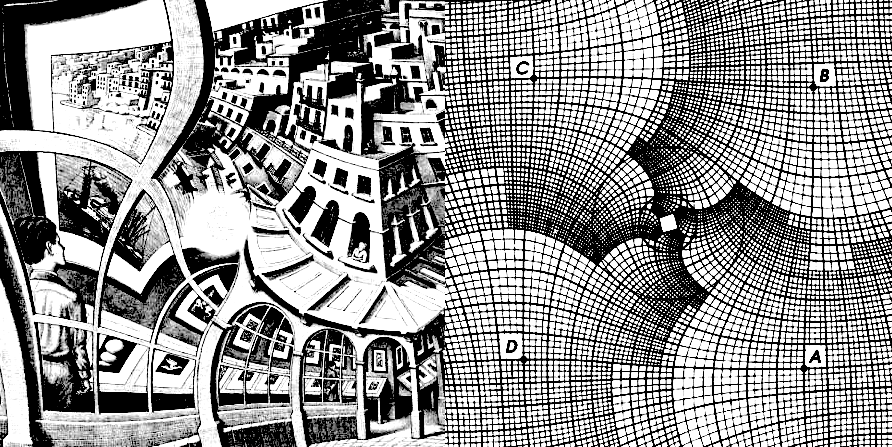
\includegraphics[height=8cm]{figures/bubbles/combined}
\caption{Escher's "Print Gallery" lithograph alongside his working sketch of the vortex-grid geometry the work was built on. On the left of the lithograph, an observer examines a framed painting of a town. Going clockwise, we see more details of the town, which has in it a print gallery, within which is the original observer. The missing centre of the piece where Escher signed the work obscures what would have been infinite nesting; the right-hand-side of the frame would have spiraled along the vortex infinitely. Treating the frame as a container, here we have an example of a container that contains itself, where movement clockwise indicates going down a level, clockwise going up, yet no explicit infinities anywhere.}
\label{fig:gallery}
\end{figure}

The space in which such an arrangement can be realised is the same as that of the Penrose staircase: splitting the lithograph into four corners, each is a locally consistent snapshot, each gluing of quadrants is a consistent (as/de)scent, but the overall manifold obtained needs to be embedded in a higher dimension. While this in principle solves the problem of finitely representing infinite descent, these kinds of spaces are not grounded in physical, embodied intuitions. I think it is mathematically neat that there can exist topological models for such modal verbs, but whether such proposals are to be taken seriously as modelling cognition is a thorny matter I don't want to say more about.